\documentclass[output=paper]{LSP/langsci}  
\author{Andrea Mathussek\affiliation{Albert-Ludwigs-University Freiburg}} 
\title{On the problem of field worker isoglosses}
\abstract{As a number of authors have already shown, the traditional approach of collecting and transcribing speech material in direct investigations may lead to differences in the data that actually do not represent diatopic variation but are based on individual transcription habits of different field workers involved. If such differences result in isoglosses separating not speech areas but different field workers’ investigation areas (“field worker isoglosses”), researchers run the risk of mapping organizational structures of projects instead of truly linguistic similarity or difference. The following article shows how dialectometric analysis can be used to visualize field worker phenomena in speech data using the example of the \textit{Sprachatlas von Mittelfranken} (SMF), which is part of the \textit{Bavarian Speech Atlas}.
}

\maketitle 
\begin{document}

% \title{}
% \author{\\
% Albert-Ludwigs-University Freiburg}
% 
% On the problem of field worker isoglosses
% \vskip11pt
% Andrea Mathussek\\
% 

\section{Definition: field worker isogloss (FWI)}
To define the concept of {\textquotedbl}field worker isogloss{\textquotedbl} (FWI) one has to start by explaining the term {\textquotedbl}isogloss{\textquotedbl}. Isoglosses are usually characterized as boundary lines between two dialect realizations of a linguistic phenomenon (cf. \citealt[296--297]{gluck_metzler_2005}). An isogloss – or sometimes only a bundle of more than one isogloss – then forms the border of a speech area in traditional dialect geography. The phenomenon is illustrated in Figure~\figref{fig:1}. Here, the different colors of the speech bubbles symbolize the different realizations of the linguistic variable under investigation and the blue line stands for the isogloss.

\begin{figure}

\includegraphics[width=0.7\textwidth]{illustrations/mathus_fig1}
\caption{Schematic layout of the concepts {\textquotedbl}isogloss{\textquotedbl} and {\textquotedbl}fieldworker isogloss{\textquotedbl}}
\label{fig:1}
\end{figure}

Based on this concept, FWIs can be defined as boundary lines between two different written interpersonal realizations in phonetic transcription, given that there is no variety in the audio data under investigation. Field worker isoglosses are thus boundary lines between two field worker areas. The illustration on the right in Figure~\figref{fig:1} exemplifies this.

A (fictitious) example might be the realization of the vowel in \textit{Frosch} ({\textquotesingle}frog{\textquotesingle}), which may be pronounced [u:] by the informants from both villages. This is symbolized by the usage of red color for both speech bubbles. The particularity now lies in the fact that despite the consistency of the informants{\textquotesingle} speech the field workers differ in their phonetic transcription and write down two different phonetic symbols, which is illustrated by the use of different colors for the note pads.\footnote{\ Phonetic transcription is always only a model for reality. Version A and B may also differ in the degree of accuracy. This may lead e. g. to one field worker marking nasalization or lenition – the other one leaving that unmarked. Differing transcriptions do not always mean that somebody made a mistake. (cf. \citealt[41--69]{mathussek_sprachraume_2014})}

It might be expected that field worker phenomena only occur rarely – especially because the problem is well known in dialectology (cf. \citealt[59--73]{hotzenkocherle_einfuhrung_1962}). Unfortunately, it appears that the problem occurs more often than expected.

In this paper I will try to explain – based on the example of the Middle Franconian Speech Atlas (SMF) – how field worker effects can find their way into linguistic data and analysis. While there are a number of established practices used by project members to avoid this problem, even atlases published in the last 10 years betray traces of individual field workers{\textquotesingle} influence. I will then show how dialectometry can be useful to discover fieldworker phenomena in transcribed corpora of linguistic data surveyed by different people in different places.

\section{The potential risk in traditional dialect atlas data}

\subsection{Example data}
The data serving as an example in this article comes from the \textit{Sprachatlas von Mittelfranken} (Dialect Atlas of Middle Franconia, SMF). This project started in 1989 and was supervised by Horst Haider Munske in Erlangen (cf. \citealt[11]{munske_zur_2013}). The map in Figure~\figref{fig:2} shows the position of the administrative district Middle Franconia in Germany marked in red. It is located in Southern Germany and anjoines Bavaria in the West.

\begin{figure}
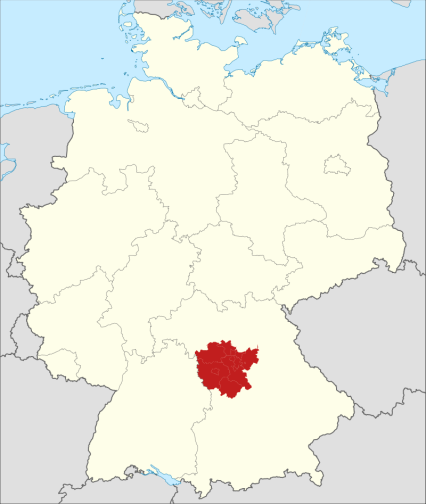
\includegraphics[width=0.3\textwidth]{illustrations/mathus_fig2}
\caption{Position of Middle Franconia in Germany (GFDL. Orginal source: \url{http://commons.wikimedia.org/wiki/File: Locator\_map\_Mittelfranken\_in\_Germany.svg})}
\label{fig:2}
\end{figure}

The region is interesting from a dialectological point of view because three High German dialects meet here: Eastern Franconian, Swabian and Northern Bavarian (cf. SMF 1: 7).

However, the Middle Franconian Atlas is only one example where such phenomena occur — other atlases using similar traditional methods would be expected to reflect transcriber-specific phenomena as well.

\subsection{Reasons for FWIs}
As Kerswill and Wright (1990: 273) describe it: {\textquotedbl}Transcription is a messy thing{\textquotedbl} \citep[273]{kerswill_limits_1990}. I will try to apply that statement to the specifics of the SMF on the following pages.

The Middle Franconian Atlas – like most of the regional dialect atlases of the 20th century – is an atlas of the so-called 2nd generation. That means that direct investigation was used as a method to collect data.\footnote{\ For the direct method, a {\textquotedbl}trained fieldworker makes on-location recordings and works through a comprehensive questionnaire with the informant. […] The investigator and the informant are united in the attempt to unearth the oldest accessible form at a particular location […].{\textquotedbl} \citep[502]{konig_investigating_2010}} Typically, atlases of this type are monodimensional atlases\footnote{\ Mono-dimensional atlases, in contrast to two-dimensional atlases, do not take pragmatic or social variation into account. (cf. \citealt{bellmann_mittelrheinischer_????} Institut für Geschichtliche Landeskunde an der Universität Mainz (ed.): Mittelrheinischer Sprachatlas; \url{http://www.igl.uni-mainz.de/service/impressum.html}, 2015/05/20)} with a few exceptions. The interviews took place in the informants{\textquotesingle} living rooms and were usually recorded on cassettes. However, the audio material was used as a reference source in problematic cases rather than as the basis for analysis. Instead, the basis for analysis consisted of the questionnaire and the handwritten phonetic transcriptions the field worker noted immediately after the informant answered a question.

Figure~\figref{fig:3} shows a part of one page from the Middle Franconian questionnaire. The {\textquotedbl}questions{\textquotedbl} are printed in the left column. They are sometimes real questions like in number 6 {\textquotedbl}How do you call it when a cow does not give any milk for some time before she calves?{\textquotedbl} The answer here can be translated literally as {\textquotedbl}stands dry{\textquotedbl} and is written down in Theutonista in the right column by the field worker. This happens virtually {\textquotedbl}on air{\textquotedbl}, while the informant is waiting for the next question. It is evident that such time pressure can lead to imprecision or even mistakes. This becomes even clearer when we have a closer look at the transcription system here.

\begin{figure}
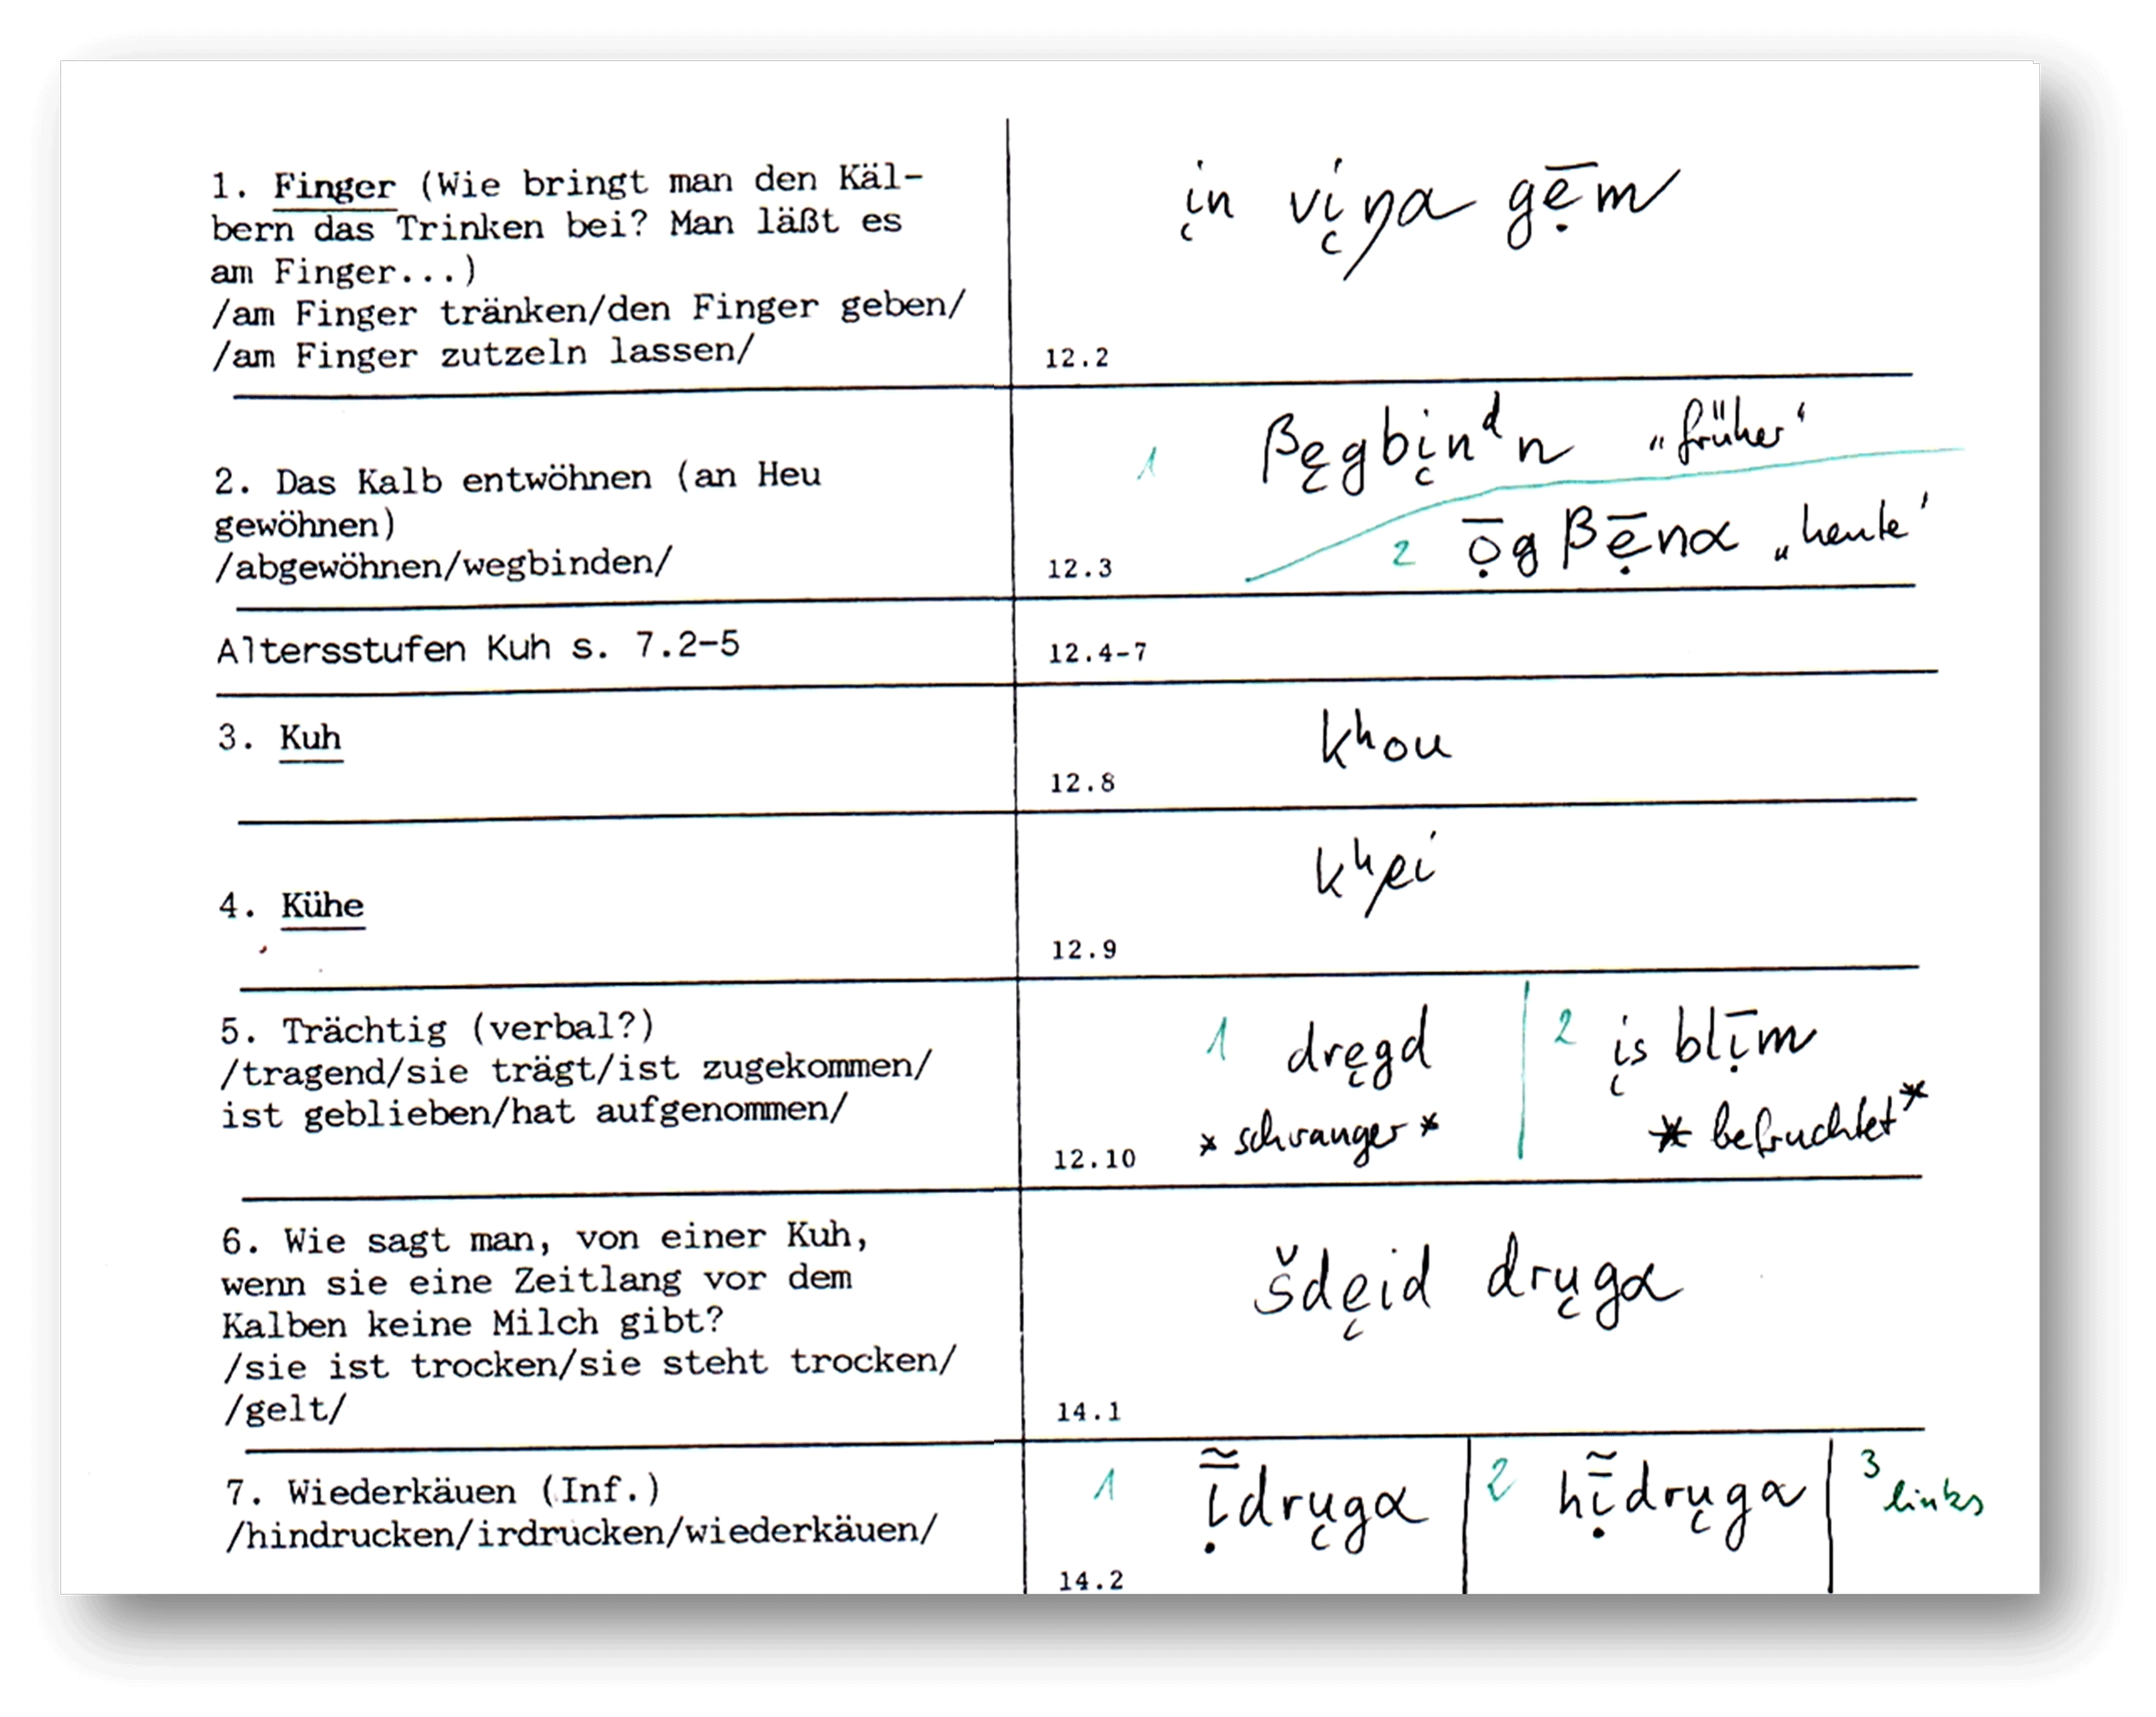
\includegraphics[width=\textwidth]{illustrations/mathus_fig3}
\caption{Original page of a SMF-questionnaire}
\label{fig:3}
\end{figure}

Figure~\figref{fig:4} shows part of the vowel diagram as it was used for the Bavarian Speech atlases. The enlarged part lists some of the possibilities to note down open fronted vowels. It becomes obvious that it is nearly impossible for two persons to write down the same symbol with exactly the same diacritics when this degree of accuracy is used. This is at least one source of possible interpersonal differences in the transcriptions.

\begin{figure}
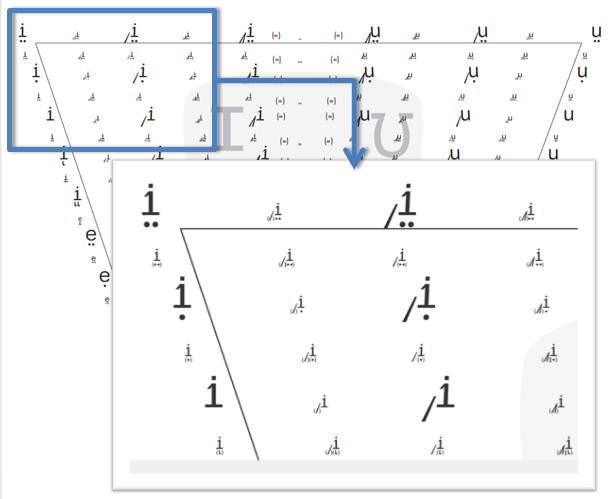
\includegraphics[width=\textwidth]{illustrations/mathus_fig4}
\caption{Part of the Theutonista vowel diagram (cf. SMF 1: 82)}
\label{fig:4}
\end{figure}

Such interpersonal variation, of course, becomes a problem, especially when more than one person is working in the field.\footnote{\ Even with one transcriber, there may be intrapersonal inconsistencies.} But division of labor is necessary, even in supposedly small areas of investigation like the administrative district of Middle Franconia, if a high density of locations is to be surveyed.

For the Speech Atlas of Middle Franconia, investigations were carried out in 167 mainly rural villages in an area of 7.000 square kilometers. In every village, about six people (men and women) served as informants – which makes a total of around 1.000 interviews with an average duration of 10 hours. The questionnaire contained 2.808 questions (cf. SMF 1: 29 ff.). It is quite clear that it is impossible for one person to manage the amount of 10.000 hours of interviews. The easiest and most economical way to split the work was to divide the area of investigation into different field workers{\textquotesingle} working sections. The field workers at the Middle Franconian Atlas, for example, lived in different areas of the administrative district or had family there – it was therefore an obvious solution to divide the area according to the field workers{\textquotesingle} locations.

\subsection{Arrangements to avoid FWIs}
It is interesting to see what measures the project members undertook to avoid the appearance of field worker phenomena. First of all, the members of the project were aware of the fact that such effects can occur in the data, as previous and neighboring projects had also alluded to the problem and suggested solutions.\footnote{\ Cf. e.\,g. \citet[59]{hotzenkocherle_einfuhrung_1962} and \citet[45]{konig_sprachatlas_1997}.} In the introductory volume, the text near the map showing the field workers{\textquotesingle} working areas (see figure 5) says: {\textquotedbl}Map 11 shows which investigations were carried out by which field worker. The field workers{\textquotesingle} individual background and the specifics of their phonetic transcriptions are given below{\textquotedbl} \citep[47]{klepsch_sprachatlas_2013}. The authors even identify and describe individual transcribing habits\footnote{\ The SDS again serves as a model here (cf. \cite[61--73]{hotzenkocherle_einfuhrung_1962}.}, which is a sign of transparency. A closer look at the description of those individual {\textquotedbl}specifics of their phonetic transcriptions{\textquotedbl} as they are described in the introductory volume will make this point even clearer. The following text is a translation of Alfred Klepsch{\textquotesingle}s characterization as a field worker:

\begin{quote}
Alfred Klepsch was born in Schwabach in 1954 and lived there from 1954 to 1961. From 1961 to 1974 he lived in Spalt, from 1974 to 1986 in Schwabach again, from 1986 to 1995 in Baiersdorf, from 1995 to 2000 in Erlangen and since then he has been living in Nuremberg. He speaks the regional dialect of the Nuremberg area. […] His transcription shows indetermination especially in the area of half-closed short vowels. From 1989 to 1992, he nearly always noted down open e-sounds [corresponds closest to æ in IPA] and o-sounds. After the coordinator M. Renn told Klepsch that the dialect variant of the Middle High German primary umlaut e has a more closed quality […] the field worker tried to close that {\textquotedbl}hearing gap{\textquotedbl}. The transcriptions of 1993, then, certainly contain some hypercorrections […]\\(\citealt[47]{klepsch_sprachatlas_2013} [translated and slightly adapted])
\end{quote}

The text deals with the background and the individual transcribing habits of Alfred Klepsch, who was the coordinator of the project. In the first paragraph it provides the reader with information about the villages in Middle Franconia Alfred Klepsch lived in and information on his speech and transcribing habits. Further below, the text names a number of other indeterminations on Klepsch{\textquotesingle}s side, which shows a really high degree of transparency. The question is: How often does a reader not only notice such texts in introductory volumes, but also use them for his or her interpretation of the data or the maps?

The members of the project did not leave the reader to work out the problem of FWI, but rather applied various methods to address this issue.

First of all, there was a lot of discussion and comparison among the sister projects (cf. \citealt[25 ff.]{klepsch_wie_2013}). The Middle Franconian Atlas is only one part of a big project comprising the whole federal state of Bavaria. Moreover, the field workers within the project always made great efforts to adjust their transcriptions. They used methods such as co-transcribing and attending each other{\textquotesingle}s test investigations, while participating in meetings and workshops. In addition there was one interview which was transcribed by all field workers. This transcription served as a reference point from then on (cf. \citealt[26]{klepsch_wie_2013}).

\begin{figure}
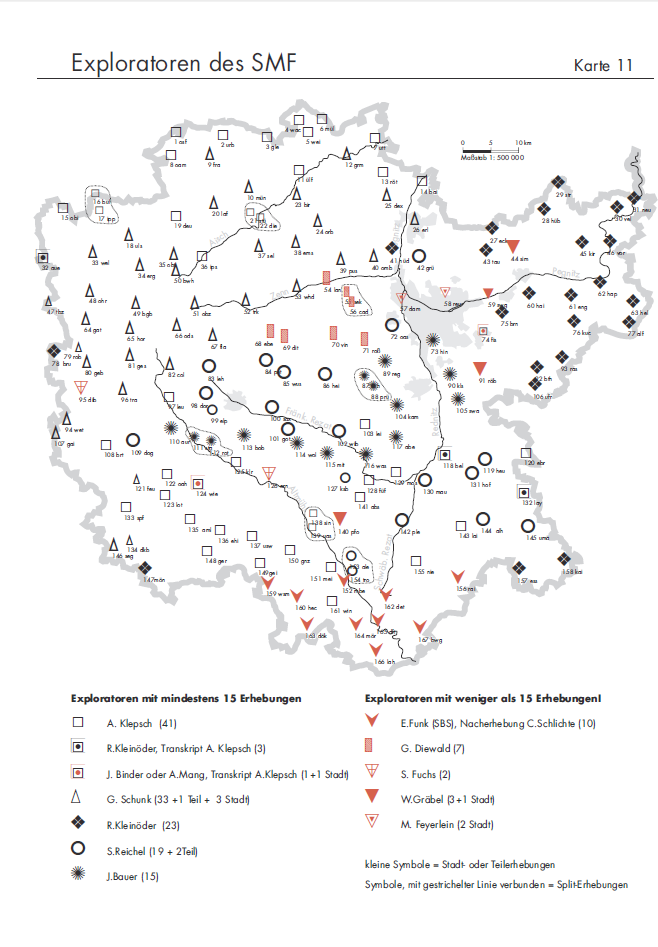
\includegraphics[width=0.9\textwidth]{illustrations/mathus_fig5}
\caption{The field workers{\textquotesingle} working sections in the SMF project (SMF 1: 48)}
\label{fig:5}
\end{figure}

Klepsch writes about the beginnings of the project in retrospective: {\textquotedbl}The comparison of the transcripts and the audio data completely puzzled the field workers. The differences between the […] transcripts were immense{\textquotedbl} \citep[25]{klepsch_wie_2013}.

Despite all the efforts he concludes: {\textquotedbl}None of the field workers achieved a level of perfection in the course of his or her career{\textquotedbl} \citep[27]{klepsch_wie_2013}.\footnote{\ As Kerswill and Wright (1990: 226) point out, a reason for this may be that transcribers use different strategies for {\textquotedbl}rationalizing and reducing to symbols the differences they have heard{\textquotedbl} (cf. \citealt[269]{kerswill_limits_1990}).}

\section{Dialectometry as a means to discover FWI}
Field worker effects are often considered something you have to expect in the data – but also something that can be addressed and dealt with when it comes to interpretation.
%%%
%%%this footnote was originally placed at the end of the section title
%%%
\footnote{\ Ogura and Wang proposed a statistical {\textquotedbl}method for clarifying fieldworker isoglosses{\textquotedbl} using the Spearman rank order correlation. They correlate the frequencies of reflexes of different ME vowels inside and outside individual investigation areas of the SED. This method seems very productive to me. Due to reasons of simplicity of the implementation of the method, I will describe another procedure to detect field worker phenomena. (cf. \citealt{ogura_isoglosses_1992}).}

It was because of this shared opinion that field worker isoglosses were not really on my mind when I was discovering speech areas and speech borders in the investigation area of Middle Franconia – using the data and material of the SMF-project (cf. \citealt{mathussek_sprachraume_2014}).

The dialectometric analysis of the realization types of 517 lexemes/phrases showed that the individual variants – irrespective of the specific statistical method in use – formed cohesive areas. The colored regions in Figure~\figref{fig:8} (not the symbols) are the result of a clustering technique (Ward{\textquotesingle}s method, 8 clusters) carried out by Gabmap.\footnote{\ Gabmap is a free {\textquotedbl}web application that visualizes dialect variation{\textquotedbl}, which was developed in Groningen. (cf. \citealt{nerbonne_gabmap_2011}.) For a description of how cluster analysis works see \url{http://www.gabmap.nl/\~app/doc/manual/clustering.html}, accessed 2015/5/21.} Figure~\figref{fig:6} shows a small part of the table that was used as a basis for the analysis with Gabmap.

\begin{figure}
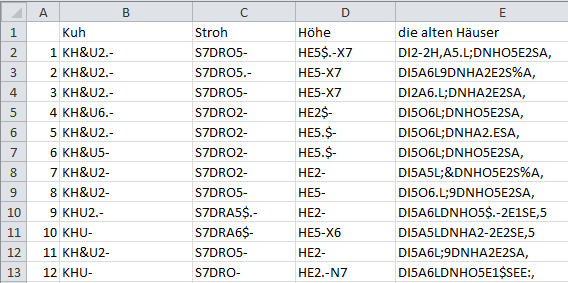
\includegraphics[width=0.9\textwidth]{illustrations/mathus_fig6}
\caption{Part of the data table prepared for the analysis with Gabmap (`cow', `straw', `height', `the old houses'; locations 1 to 12).
%%%
%%%this was originally a caption-internal footnote
%%%
The table does not show IPA or Theutonista but the so called ``Kodate'' – a code that translates the basic signs and diacritics of Theutonista into ASCII (American Standard Code for Information Interchange) (cf. \citealt[38--40]{reichel_elektronische_2013}).}
\label{fig:6}
\end{figure}

The comparison of this analysis with maps developed with traditional methods then revealed some discrepancies.

Figure~\figref{fig:7} visualizes some results of the traditional approach. I picked out about 40 Middle High German speech sounds in different sound environments and looked for different realizations in the 167 villages. The resulting isoglosses in the area of consonants are shown in black; the isoglosses for vowel phenomena are marked in red.

\begin{figure}
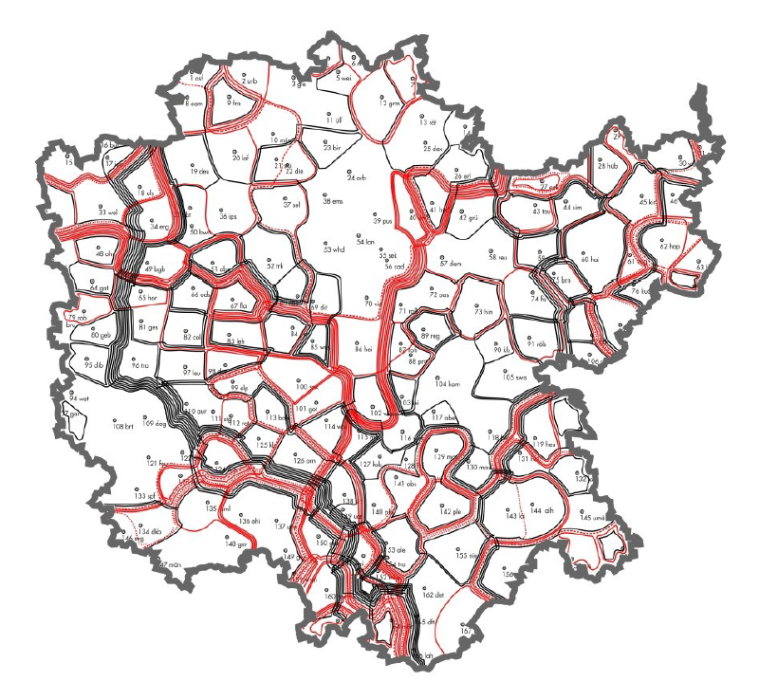
\includegraphics[width=.7\textwidth]{illustrations/mathus_fig7}
\caption{Traditional approach: Consonantal and vocalic isoglosses \citep[107]{mathussek_sprachraume_2014}.}
\label{fig:7}
\end{figure}

What attracts attention here is that besides some obvious similarities between the isoglosses in \figref{fig:7} and the areas in figure 8 – like the bundle of isoglosses along the western border of the area of investigation and the area in light orange and pink taken together – there are areas on the map in figure 8 that do not coincide with the results of the traditional analysis.

The solution to this problem is revealed when one considers the striking match between the dialectometric analysis and the investigation areas of the individual field workers. What the dialectometric analyses showed were, without much doubt, not really speech areas, but rather field worker effects in the data!

\begin{figure}
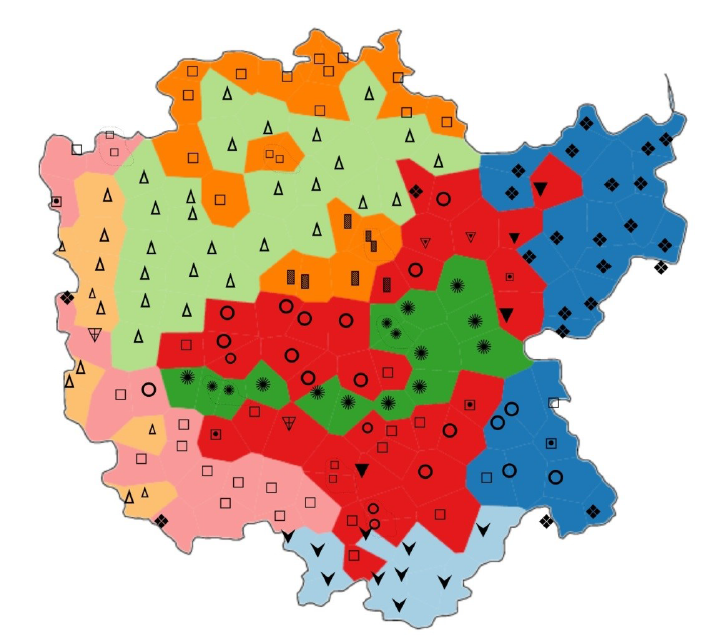
\includegraphics[width=.7\textwidth]{illustrations/mathus_fig8}
\caption{Clusters and field worker{\textquotesingle}s working sections \citep[216]{mathussek_sprachraume_2014}.}
\label{fig:8}
\end{figure}

The map in \figref{fig:8} is a blend of a Gabmap cluster map and the map in the introductory volume of the Middle Franconian Atlas showing which field worker collected data in which village (SMF 1: 48, see \figref{fig:5} above). There is a noticeable concordance of symbols and clusters on the map. In particular, the dark green and the light blue section match the symbols one-to-one, which means that exactly one field worker worked in all the villages Gabmap clustered together here as one. It was also exactly one person who was responsible for both the light green and the light orange areas, taken together.

The next task was to find out which properties of the data were responsible for the clustering – or in other words: if it was really interpersonally different transcribing habits that were so influential on the data that they marginalized the de facto existing linguistic differences. Gabmap offers a very useful tool named cluster determinants. The tool helps to identify those lexemes that are the most relevant for a cluster. That means the realization types are very similar or identical within the cluster and they rarely or never appear in other clusters.\footnote{\ Cf. \citet{nerbonne_gabmap_2011}.}

I will only give a few examples here, but more are to be found. The analysis of the cluster determinants for the light green cluster (cf. figure 8) showed that in the villages in this area, words like [o:ʃdən]\footnote{\ IPA is used here only for technical reasons. As I pointed out above, SMF and the other Bavarian speech atlases used Theutonista.} \textit{Ostern} ({\textquotesingle}easter{\textquotesingle}) and [dsɪxəd] (\textit{er}) \textit{zöge} ({\textquotesingle}he would pull{\textquotesingle}) often have the highest values in the cluster determinants{\textquotesingle} analysis. Moreover, this field worker noted down aspirated voiceless dental plosives, whereas the others didn{\textquotesingle}t. One example here is [gvidət\textsuperscript{h}] \textit{gefüttert} ({\textquotesingle}fed{\textquotesingle}). Thirdly, the field worker in this area transcribed clusters of vowels and used many diacritics, as in \textit{heiraten} ({\textquotesingle}marry{\textquotesingle}), which may look like \figref{fig:9} in Theutonista:

\begin{figure}
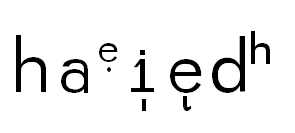
\includegraphics[width=.25\textwidth]{illustrations/mathus_fig9}
\caption{Theutonista transcription of \textit{heiraten} ({\textquotesingle}marry{\textquotesingle}).}
\label{fig:9}
\end{figure}

This was also a peculiarity that very rarely occurred in other regions.

In case of the light blue cluster in the south of Middle Franconia we find a very clear example of a field worker phenomenon. Figure~\figref{fig:10} shows the distribution of the phonetic symbol {\textless}w{\textgreater}, which stands for the bilabial fricative in Theutonista. As one can see, the area perfectly corresponds with the cluster in light blue in the south of the investigation area (cf. Figure~\figref{fig:7}). A closer look into the data shows that {\textless}w{\textgreater} only appears in transcripts from this area where two neighboring projects made investigations. The Middle Franconian Atlas got data here from the Speech Atlas of Bavarian Swabia (SBS) and they had slightly different transcription conventions there (cf. SMF 1: 30). In the rest of the investigation area the field workers used the sign {\textless}ß{\textgreater} in all of the cases where the Swabians used {\textless}w{\textgreater}. This shows a very clear case of field worker influence or even neighboring project phenomenon. However, those cases are not the dangerous ones because they can easily be figured out in the data:\footnote{\ At least when the editor takes a closer look into the data.}

%%%
%%% replace angled brackets with chevrons?
%%%
\begin{figure}
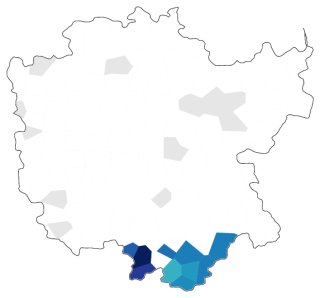
\includegraphics[width=.5\textwidth]{illustrations/mathus_fig10}
\caption{Distribution of {\textless}w{\textgreater} \citep[226]{mathussek_sprachraume_2014}.}
\label{fig:10}
\end{figure}
  
\figref{fig:10} is an example for a distribution map made with Gabmap. This feature allows the mapping of the distribution of individual items or strings of items in the data. In this case the map shows that the symbol {\textless}w{\textgreater} only occurs in those locations that were examined by members of the SBS project (light blue cluster in \figref{fig:8}).

All in all, the data analysis showed a clear correlation between the Gabmap clusters and the field workers{\textquotesingle} individual areas of investigation. In the corpus, individual transcription habits were much more relevant for the structure of the data than the de facto existing linguistic difference.

The last step was then to check the linguistic features which the cluster determinants analysis had shown were especially relevant for the structure of the data in the audio material. Of course, only a random sample could be tested here. The check confirmed the results of the dialectometric analysis: In most cases under suspicion, the differences in the transcriptions were not a matter of real linguistic variance.

To sum up, I recommend a dialectometric analysis of dialect geographical data in six steps:\footnote{\ Of course, this analysis can be done with different software, too.} Firstly, the whole corpus is mapped using a cluster technique with approximately the number of clusters that would be expected from traditional approaches. Secondly, the results should be compared (if possible) to the results of traditional approaches. In a third step, the results should be compared to the information about investigation areas and field workers that is accessible. If there are inconsistencies, or if the areas seem to correspond more to the investigation areas than to the traditional approaches (or if there is no accessible information on one of the aspects) the analysis of cluster determinants should be conducted to find out about the lexemes or phrases that are mostly {\textquotedbl}responsible{\textquotedbl} for the clusters in a fourth step. The results of this analysis can be checked with distribution maps (fifth step), before in a sixth step certain features should be examined in the audio data.

\section{FWIs on actual maps in the printed atlases?}
Subsequently, an important question to ask was to what extent this had influenced the maps and results in the printed volumes of the atlases. The following two short examples show that field worker phenomena even made it into the printed volumes.\footnote{\ It{\textquotesingle}s easier to discover field worker phenomena in the volumes of the SBS, where the members decided to print investigation areas on every base map. This enables a quick check whether feature isoglosses correlate or not with boundaries of fieldworker areas (cf. SBS 1: 45). Due to the fact that 13 people worked as field workers for the SMF (SMF 1: 48) project (but only 3 for SBS, SBS 1: 45), the investigation areas are not printed on the base map in the Middle Franconian Atlas.}

The first example can be found in map 45 in volume 4 of the Middle Franconian Atlas. It deals with the realizations of Middle High German t in the position between -s- and -en as in the lexemes \textit{Bürste} ({\textquotesingle}brush{\textquotesingle}), \textit{Fenster} ({\textquotesingle}window{\textquotesingle}), \textit{Gerste} ({\textquotesingle}barley{\textquotesingle}) and \textit{Husten} ({\textquotesingle}cough{\textquotesingle}). The green line around the investigation area of the field worker Johannes Bauer in figure 10 corresponds perfectly to the area where reduced plosives were plotted on the map. Nowhere else in the area of investigation had field workers noted down reduced plosives. The unique shape of the area makes it hard to believe that the concordance is only accidental.

\begin{figure}
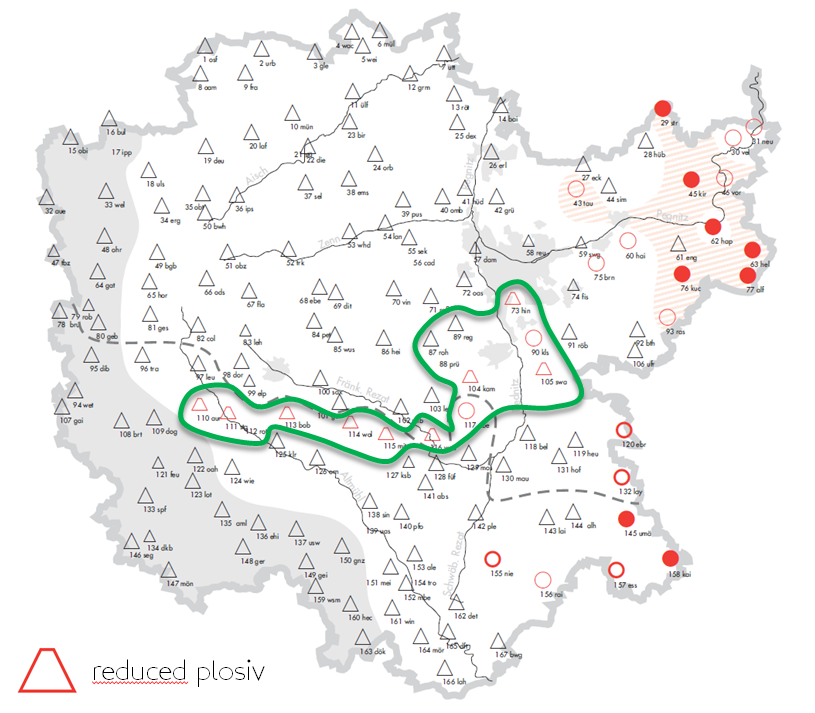
\includegraphics[width=.7\textwidth]{illustrations/mathus_fig11}
\caption{Field worker effects in SMF 1, map 45: MHG t in the position between -s- and -en and one individual field worker{\textquotesingle}s working area (in green) (cf. \citealt[240]{mathussek_sprachraume_2014}).}
\label{fig:11}
\end{figure}

The second example (see \figref{fig:11}) is taken from the second volume of the Middle Franconian Atlas and refers to the realizations of the vowel in the demonstrative pronoun \textit{die} (meaning {\textquotesingle}this{\textquotesingle} or {\textquotesingle}these{\textquotesingle}). This part of map 100 is intended to illustrate the border between a realization type {\textquotedbl}closed vowel{\textquotedbl} and a realization type {\textquotedbl}neutral or open vowel{\textquotedbl}. I drew an isogloss between the two types and compared it to the border between Alfred Klepsch{\textquotesingle}s (orange) and Gunter Schunk{\textquotesingle}s (light green) investigation area. There is a one-to-one match between the two borders – despite the fact that its progression is quite unique.

\begin{figure}
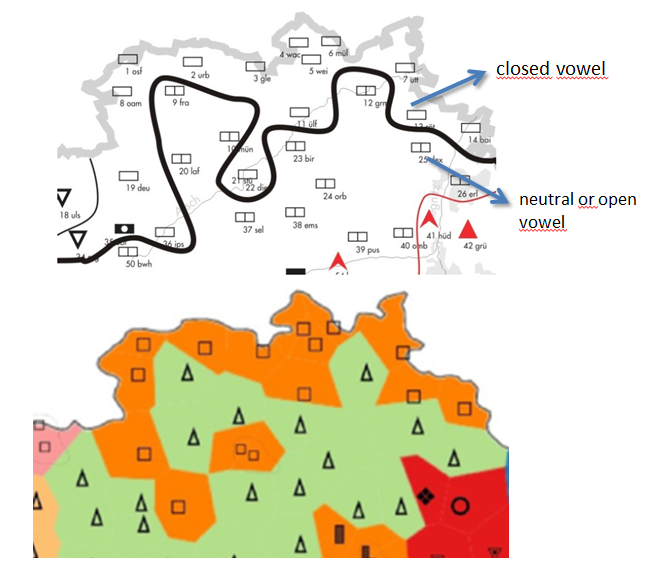
\includegraphics[width=.4\textwidth]{illustrations/mathus_fig12}
\caption{Field worker effects in SMF 2, map 100: Realization of the vowel in the demonstrative pronoun \textit{die} \citep[241]{mathussek_sprachraume_2014}.}
\label{fig:12}
\end{figure}

Those are only two examples, but it is quite certain that there are more – and not only in the Middle Franconian Atlas. In both cases mentioned above, audio data was checked for reference. It was not possible to identify any differences between the dialect realizations inside and outside the clusters.

Field worker isoglosses, then, are present in speech atlases and are presented as {\textquotedbl}real isoglosses{\textquotedbl} separating speech variants.

\section{Implications}
The findings of this analysis lead to a few implications.

First of all, it is important for anyone working with speech atlases in which different field workers were responsible for collecting the data to pay attention to the field workers{\textquotesingle} individual areas of investigation. That, of course, may not always be possible or easy because the degree of transparency varies a lot from atlas to atlas.

Despite that fact, the search for field worker phenomena has to be carried out systematically and needs to be expanded to other atlas projects and their maps and data. Therefore, dialectometric approaches can be used to explore the data and to identify the relevant features in the data.

Furthermore, the findings show that the analysis of huge amounts of data does not make traditional approaches redundant. That does not mean that dialect geographers have to lean over hand-drawn maps again – Gabmap offers tools for {\textquotedbl}traditional{\textquotedbl} methods, too – but a close look into the data is absolutely necessary.

A last point concerns the question of the degree of details in phonetic transcription. Do we really need all those diacritics if it is seemingly impossible for two people to use them in the same way?

Here, more modern approaches and methods of investigation seem to provide help. For the project {\textquotedbl}Effects of the national border on the linguistic situation in the Upper Rhine Area{\textquotedbl} (Frontière linguistique au Rhin Supérieur, FLARS) for example, there were no transcripts made in the actual investigation situation, but the researchers only transcribed relevant parts later with the help of the audio data (cf. \citealt{auer_auswirkungen_2015}).\footnote{\ Cf. also the note on Hammarström{\textquotesingle}s method of \textit{transcription phonétique indirecte} ({\textquotesingle}subsequent transcription of audio material under laboratory conditions{\textquotesingle}) in \citet[73]{hotzenkocherle_einfuhrung_1962}.} This leads to a closer relation between audio data and analysis; the process of (phonetic) transcribing is carried out by one person\footnote{\ This method, of course, does not solve the problem of {\textquotedbl}within-transcriber variability{\textquotedbl} \citep[258]{kerswill_limits_1990}.} in a relatively short time, and the focus is on the aspect that will be the object of analysis.

\printbibliography[heading=subbibliography,notkeyword=this]
\end{document}